\documentclass{article}

\usepackage{microtype}
\usepackage{graphicx}
\usepackage{subcaption}
\usepackage{booktabs}
\usepackage{hyperref}
\usepackage{amsmath}
\usepackage{amssymb}
\usepackage{mathtools}
\usepackage{placeins}
\usepackage{tikz}
\usepackage{pgfplots}
\usepackage{multirow}
\pgfplotsset{compat=1.18}
\usetikzlibrary{arrows.meta,shapes.geometric,positioning,calc,fit,backgrounds}
\usepackage[capitalize,noabbrev]{cleveref}
\usepackage{icml2026}

\icmltitlerunning{Evidence-Gated Memory}

\begin{document}

\twocolumn[
\icmltitle{Evidence-Gated Memory for Token-Efficient Frozen LLM Agents}

\begin{icmlauthorlist}
\icmlauthor{Anonymous Authors}{anon}
\end{icmlauthorlist}
\icmlaffiliation{anon}{Anonymous Institution}
\icmlcorrespondingauthor{Anonymous Authors}{anonymous@example.com}
\icmlkeywords{evidence-gated memory, long-term memory, LLM agents, retrieval, token efficiency, efficient agents}

\vskip 0.3in
]

\printAffiliationsAndNotice{}

\begin{abstract}
Long-horizon agents can spend many reader tokens on stale or redundant retrieved memories. We study \emph{evidence-gated memory}, a compact post-retrieval gate layered over the official open-source Mem0 package. The gate preserves Mem0's ranked evidence, applies a conservative stale-evidence guard, and caps reader context to a smaller top-$k$. On 311 LongMemEval questions, ODV2 compact reduces reader tokens by 42.7\%, retrieved context tokens by 59.1\%, and retrieved items by 58.7\%, while changing accuracy from 62/311 (19.9\%) to 58/311 (18.6\%). This lowers reader tokens per correct answer from 2{,}444 to 1{,}497; the top-5 baseline buys four additional aggregate correct answers for 64{,}720 extra reader tokens. A same-budget top-2 replay reaches 54/311, while top-3 reaches 60/311 at higher cost. These results are a constrained-budget token-savings ablation, not a reproduction of Mem0 platform accuracy or evidence that ODV2 improves answer quality.
\end{abstract}

\section{Introduction}

Long-horizon agents increasingly depend on external memory to carry information across sessions, tools, and user interactions. Existing retrieval-centered systems are effective when the main challenge is recovering relevant evidence. They are less direct when the challenge is state maintenance: a user moves, changes a preference, corrects a prior statement, or reverts to an earlier value. In these cases, the memory layer may retrieve both the old and new versions of a fact, forcing a frozen reader to infer which value remains valid.

This paper asks a narrower systems question: can an evidence-gated memory layer reduce the amount of context passed to a frozen reader while keeping answer behavior close to an existing memory backend? We keep the reader, prompt template, and decoding configuration fixed, and vary only whether an ODV2 evidence gate is placed after official open-source Mem0 retrieval. Our hypothesis is that token-efficient memory should be allowed to compact evidence, but only under conservative gates. A memory layer should avoid injecting replacement facts and should avoid suppressing evidence unless the retrieved records themselves make the edit low-risk.

We evaluate this idea on LongMemEval~\cite{wu2025longmemeval}, a benchmark designed around long-term interactive memory. Our target method overlays a write-time evidence-state ledger on top of the official Mem0 OSS package~\cite{chhikara2025mem0}. Earlier broad pruning variants were too aggressive. The current policy is deliberately narrower: Mem0 remains the retrieval backbone, ODV2 never injects ODV2-only evidence into the reader prompt, and the compact gate primarily tests whether a small ranked subset of Mem0 evidence can preserve paired behavior while lowering token spend.

The completed run covers knowledge-update, single-session-preference, multi-session, and single-session-user, for 311 paired questions. The compact gate reduces reader-token budget substantially in every category, with a final accuracy difference of $-4$ correct answers relative to official Mem0 OSS. The resulting budget tradeoff is large: official Mem0 spends 151{,}558 reader tokens for 62 correct answers, whereas the compact gate spends 86{,}838 reader tokens for 58 correct answers. We additionally replay official Mem0 with top-$k$ values from 1 through 4, producing naive truncation baselines that isolate whether the result is simply fewer retrieved records. This framing is important: the result is not a benchmark-level Mem0 accuracy claim. It is a paired cost-reduction test under a constrained open-source Mem0 setup.

\paragraph{Contributions.}
We make three contributions. First, we define a conservative post-retrieval evidence-gating interface that layers current/archive/conflict state over an existing memory backend without replacing its ranked retrieval. Second, we instantiate the interface for the official open-source Mem0 package using a compact top-$k$ gate and a stale-evidence guard. Third, we provide paired LongMemEval evidence showing large reader-context reductions, while explicitly treating accuracy as a guardrail and separating evidence-gated compaction from plain top-$k$ Mem0 replay baselines.

\section{Related Work}

Retrieval-augmented generation shows that non-parametric memory can improve a frozen model by supplying external evidence~\cite{lewis2020rag}. Persistent-agent systems extend this idea to long-lived interaction. Generative Agents store observations and reflections~\cite{park2023generative}; MemGPT treats memory management as an operating-system-like problem~\cite{packer2023memgpt}; and Mem0 provides a scalable long-term memory substrate for production agents~\cite{chhikara2025mem0}. These systems make external memory a practical adaptation mechanism, but they do not fully separate evidence recall from evidence budgeting.

Long-term memory benchmarks make that distinction important. LoCoMo evaluates very long-term conversational memory~\cite{maharana2024locomo}, and LongMemEval focuses on interactive assistant memory across sessions~\cite{wu2025longmemeval}. Many failures in these settings arise because evidence changes over time: a retrieved span can be relevant but stale. Our work treats revision, reversion, conflict, and current-state selection as first-class memory operations.

This design is related to belief revision~\cite{alchourron1985logic}, but implemented as an engineering layer for LLM agents rather than a symbolic knowledge base. It is also aligned with efficient adaptation. Parameter-efficient tuning and continual-learning methods adapt model weights~\cite{hu2022lora,wang2024comprehensive}, whereas memory-state updates can be cheaper when the change is user-specific or short-lived. This is consistent with Green AI arguments for preferring lower-cost mechanisms when quality is preserved~\cite{strubell2019energy,schwartz2020green}.

\section{Method}

\subsection{Memory State}

Each memory record contains an entity, attribute, value, timestamp, scope, provenance fields, and an evidence status. The status is one of \{\textsc{Active}, \textsc{Reinforced}, \textsc{Superseded}, \textsc{Conflicted}, \textsc{Archived}\}. The memory system maintains four stores: an append-only episodic log, a current-state store keyed by $(\textit{entity}, \textit{attribute})$, an archive of superseded or low-confidence entries, and a conflict table for unresolved same-key contradictions.

Incoming structured facts are classified into revision operations: \textsc{Add}, \textsc{Reinforce}, \textsc{Revise}, \textsc{Revert}, \textsc{Split\_Scope}, \textsc{Conflict\_Unresolved}, \textsc{Low\_Confidence}, or \textsc{No\_Op}. A revision moves the previous active value into the archive and installs the new value in current state. A reversion does the same, but records that the new value was previously observed. Conflicts are not silently resolved; they are held in the conflict table.

\begin{figure}[t]
\centering
\resizebox{0.96\columnwidth}{!}{%
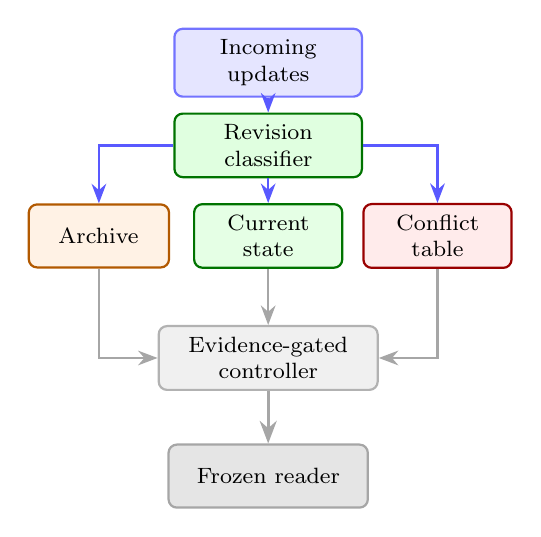
\begin{tikzpicture}[
    >=Stealth,
    box/.style={rectangle, draw, rounded corners=3pt, minimum height=0.8cm,
                font=\footnotesize, align=center, inner sep=4pt, line width=0.8pt},
    ingest/.style={box, fill=blue!10, draw=blue!55, text width=2.1cm},
    classifier/.style={box, fill=green!12, draw=green!45!black, text width=2.1cm},
    archive/.style={box, fill=orange!10, draw=orange!70!black, text width=1.5cm},
    current/.style={box, fill=green!10, draw=green!45!black, text width=1.6cm},
    conflict/.style={box, fill=red!8, draw=red!60!black, text width=1.6cm},
    query/.style={box, fill=gray!12, draw=gray!60, text width=2.5cm},
    reader/.style={box, fill=gray!20, draw=gray!70, text width=2.25cm},
    arr/.style={->, line width=0.9pt, draw=gray!70}
  ]
  \node[ingest] (u) at (0,1.25) {Incoming updates};
  \node[classifier] (c) at (0,0.2) {Revision classifier};
  \node[archive] (a) at (-2.15,-0.95) {Archive};
  \node[current] (s) at (0,-0.95) {Current state};
  \node[conflict] (f) at (2.15,-0.95) {Conflict table};
  \node[query] (p) at (0,-2.5) {Evidence-gated controller};
  \node[reader] (r) at (0,-4.0) {Frozen reader};

  \draw[arr, draw=blue!65] (u) -- (c);
  \draw[arr, draw=blue!65] (c) -- (s);
  \draw[arr, draw=blue!65] (c) -| (a);
  \draw[arr, draw=blue!65] (c) -| (f);
  \draw[arr] (s) -- (p);
  \draw[arr] (a) |- (p);
  \draw[arr] (f) |- (p);
  \draw[arr, line width=1.15pt] (p) -- (r);
\end{tikzpicture}
}
\caption{ODV2 maintains explicit evidence state at write time, but query-time edits are conservative and evidence-gated.}
\label{fig:framework}
\end{figure}

\subsection{Official Mem0 Compact Gate}

Let $B_5(q)$ be the top five records returned by official Mem0 OSS for query $q$. The compact ODV2 policy starts from this ranked Mem0 output and performs no independent retrieval into the reader prompt. ODV2 maintains its own current-state and archive stores while Mem0 ingests the same context, but query-time evidence remains anchored to Mem0. This choice keeps the comparison focused on whether an evidence gate can reduce the reader context without changing the underlying memory backend or answerer.

\paragraph{Stale-state guard.}
For current-state queries, ODV2 may remove a stale same-key record only if all of the following are true: (1) the current-state store contains a decisive value for the query key; (2) the current value is already present in $B_5(q)$; (3) the archive contains an older same-key value; and (4) the retrieved stale record matches that archived older value. This is intentionally asymmetric: ODV2 never injects evidence that Mem0 did not retrieve, and it never removes a stale value unless Mem0 has already retrieved the corresponding current value.

\paragraph{Compact ranked context.}
After the stale-state guard, the policy preserves Mem0's ranking and returns at most the first two remaining records to the reader. The compact policy can therefore be written as
\begin{equation}
\begin{aligned}
B'(q) = \operatorname{top}_2(&B_5(q) \setminus \\
&\{r : g(q, r, B_5(q), C(q), A(q)) = 1\}),
\end{aligned}
\end{equation}
where $C(q)$ and $A(q)$ are the current and archive entries for $q$, and $g$ is true only when the observable gates above certify archived stale state. This differs from broad state pruning and from ODV2-first retrieval. The controller is designed for low-cost filtering over Mem0's own evidence, not for maximizing standalone recall.

\section{Evaluation}

We evaluate on LongMemEval~\cite{wu2025longmemeval}. The baseline is \texttt{official\_mem0}, an adapter around the official open-source Mem0 package. The comparison policy is \texttt{official\_mem0\_odv2\_selective} in compact gate mode with compact top-$k=2$. The baseline retrieves five Mem0 records per query; the compact gate returns at most two ranked Mem0 records after the conservative stale-state guard. To isolate whether the result is merely top-$k$ truncation, we also replay \texttt{official\_mem0} diagnostics through the same frozen reader using only the first $k \in \{1,2,3,4\}$ Mem0 records. These replays do not rerun Mem0 extraction or ODV2 state maintenance. We report paired comparisons on four LongMemEval categories: knowledge-update ($N=78$), single-session-preference ($N=30$), multi-session ($N=133$), and single-session-user ($N=70$), for 311 total questions.

The Mem0 extraction LLM is \texttt{Qwen/Qwen2.5-7B-Instruct} served through vLLM with a 16k serving context, bfloat16 weights, add batch size 16, 2000 maximum message characters, and raw fallback disabled to avoid invalid empty-memory runs. The Mem0 embedder is \texttt{sentence-transformers/all-MiniLM-L6-v2} with local Qdrant storage. The frozen reader is also \texttt{Qwen/Qwen2.5-7B-Instruct}, evaluated with the repository local-Hugging Face backend, bfloat16 inference, inference batch size 64, reader flush size 8, and an 8192-token reader context window. Both policies use the same cleaned input file, \texttt{data/longmemeval\_s\_cleaned.json}, and the same reader prompt template.

Primary metrics are prompt tokens, reader total tokens, retrieved context tokens, and retrieved item count. Accuracy, paired wins, and paired losses against \texttt{official\_mem0} are reported as guardrail metrics to show how much answer behavior changes under compaction. Pairing is by LongMemEval case id, so a win means the compact gate is correct where the baseline is incorrect, and a loss means the reverse. Accuracy uses a local span-match proxy rather than the official leaderboard protocol: normalized exact match or normalized span match after lowercasing, article removal, punctuation removal, and whitespace normalization. The results therefore should not be compared directly to Mem0 platform or leaderboard numbers, which use different Mem0 backends, larger retrieval depths, and different evaluation harnesses~\cite{mem0benchmarks2026}.

For systems sanity checking, we also run a cache-free reader-only replay on a deterministic 64-case subset shared by official Mem0, ODV2 compact, top-2, and top-3. This replay disables the response cache and reuses the already-retrieved records, so it measures frozen-reader wall-clock cost without rerunning Mem0 ingestion or extraction. Finally, we run an oracle answer-session replay on 64 cases by giving the reader only LongMemEval sessions marked as containing the answer. This is not a memory policy, but it tests whether the local reader and span scorer can solve cases when focused answer evidence is present.

\paragraph{Scope of the run.}
The experiment is intended as an efficiency ablation under a constrained OSS Mem0 reader budget, not as a reproduction of the published Mem0 platform result. The relevant question is paired: given the same OSS Mem0 extraction run and the same frozen reader, how much context can the ODV2 gate remove before accuracy changes? This design makes token savings directly interpretable, but it also explains the low absolute accuracy observed in the current run.

\section{Results}

\begin{table*}[t]
\caption{LongMemEval results for the official Mem0 OSS compact-gate run. $\Delta$Prompt is ODV2 compact minus official Mem0. Wins are cases where ODV2 is correct and Mem0 is wrong; losses are the reverse. \texttt{Top2} is a replay of the same Mem0 retrieved records with only the first two records passed to the reader.}
\label{tab:aggregate_results}
\vskip 0.15in
\begin{center}
\begin{small}
\begin{sc}
\begin{tabular}{lccccccc}
\toprule
Category & $N$ & Mem0 Acc & ODV2 Acc & Top2 Acc & $\Delta$Prompt & Win & Loss \\
\midrule
Knowledge-update & 78 & 25/78 (.321) & 23/78 (.295) & 23/78 (.295) & $-45.00\%$ & 1 & 3 \\
\midrule
Single-sess-pref & 30 & 0/30 (.000) & 0/30 (.000) & 0/30 (.000) & $-46.00\%$ & 0 & 0 \\
\midrule
Multi-session & 133 & 7/133 (.053) & 7/133 (.053) & 4/133 (.030) & $-44.65\%$ & 6 & 6 \\
\midrule
Single-sess-user & 70 & 30/70 (.429) & 28/70 (.400) & 27/70 (.386) & $-43.86\%$ & 1 & 3 \\
\midrule
Total & 311 & 62/311 (.199) & 58/311 (.186) & 54/311 (.174) & $-44.70\%$ & 8 & 12 \\
\bottomrule
\end{tabular}
\end{sc}
\end{small}
\end{center}
\vskip -0.1in
\end{table*}

\begin{table*}[t]
\caption{Efficiency and top-$k$ sensitivity over 311 paired cases. Reader-token changes are relative to official Mem0 top-5. Tokens per correct answer and correct answers per 100k reader tokens are cost-normalized utility metrics; they are not accuracy metrics.}
\label{tab:token_budget}
\vskip 0.15in
\begin{center}
\begin{tiny}
\begin{sc}
\begin{tabular}{lcccccc}
\toprule
Policy & Records & Correct & Reader tok. & $\Delta$ tok. & Tok./correct & Correct/100k \\
\midrule
\texttt{official\_mem0\_top1} & 1 & 50/311 & 65{,}812 & $-56.58\%$ & 1{,}316 & 76.0 \\
\texttt{official\_mem0\_top2} & 2 & 54/311 & 86{,}002 & $-43.25\%$ & 1{,}593 & 62.8 \\
\texttt{official\_mem0\_odv2} & $\leq$2 & 58/311 & 86{,}838 & $-42.70\%$ & 1{,}497 & 66.8 \\
\texttt{official\_mem0\_top3} & 3 & 60/311 & 110{,}058 & $-27.38\%$ & 1{,}834 & 54.5 \\
\texttt{official\_mem0\_top4} & 4 & 59/311 & 130{,}157 & $-14.12\%$ & 2{,}206 & 45.3 \\
\texttt{official\_mem0} & 5 & 62/311 & 151{,}558 & --- & 2{,}444 & 40.9 \\
\bottomrule
\end{tabular}
\end{sc}
\end{tiny}
\end{center}
\vskip -0.1in
\end{table*}

\begin{table}[t]
\caption{Mechanism attribution on the 311 paired ODV2 cases. The measured savings are dominated by ranked context compaction, not by frequent stale-state deletion.}
\label{tab:mechanism_attribution}
\vskip 0.15in
\begin{center}
\begin{scriptsize}
\begin{sc}
\begin{tabular}{lr}
\toprule
Diagnostic & Count \\
\midrule
Paired ODV2 rows & 311 \\
Compact-mode rows & 303 \\
Non-compact rows & 8 \\
Stale records removed by guard & 2 \\
Mem0 ranked records omitted by compaction & 907 \\
ODV2-only records appended & 0 \\
\bottomrule
\end{tabular}
\end{sc}
\end{scriptsize}
\end{center}
\vskip -0.1in
\end{table}

\paragraph{Accuracy guardrail.}
Across the 311 paired cases, official Mem0 OSS answers 62 cases correctly, while the ODV2 compact gate answers 58 correctly. The paired accuracy difference is therefore $-4$ cases, or $-1.3$ percentage points. There are 8 paired wins for ODV2 and 12 paired losses; 50 cases are correct for both methods and 241 are wrong for both. The largest absolute category is multi-session, where both methods are tied at 7/133, but single-session-user and knowledge-update each contribute a two-case deficit for ODV2.

\paragraph{Reader-budget reduction.}
The token-savings signal is the central result. ODV2 compact reduces prompt tokens by 44.70\%, total reader tokens by 42.70\%, retrieved context tokens by 59.07\%, and retrieved items by 58.65\%. The run logs show compact-mode behavior on 303 of 311 paired ODV2 rows, with two stale-value removals and 907 ranked Mem0 records omitted by compaction. Thus the present evidence supports ODV2 as an evidence-gated token-budget controller, not as an accuracy-improving retriever.

\paragraph{Cost-normalized utility.}
Because the goal is token savings under an accuracy guardrail, the most direct utility view is reader tokens spent per correct answer. Official Mem0 top-5 spends 151{,}558 reader tokens for 62 correct answers, or 2{,}444 reader tokens per correct answer. ODV2 compact spends 86{,}838 reader tokens for 58 correct answers, or 1{,}497 tokens per correct answer. Equivalently, the top-5 baseline pays 64{,}720 additional reader tokens to recover four additional aggregate correct answers, a marginal cost of 16{,}180 reader tokens per extra correct answer. Top-1 has the lowest token cost per correct answer but answers only 50 cases correctly; among operating points with at least 58 correct answers, ODV2 has the lowest token cost per correct answer.

A paired bootstrap over 20{,}000 case resamples gives a 95\% interval of 41.9--43.4\% for reader-token reduction and 28.6--47.1\% for tokens-per-correct reduction. The same bootstrap gives an accuracy-delta interval of $-4.18$ to $+1.61$ percentage points, reinforcing that accuracy should be treated as a guardrail rather than an improvement claim.

\paragraph{Manual scorer audit.}
We reviewed a 50-case audit sample, giving 100 policy-case judgments across official Mem0 and ODV2 compact. Manual review agrees with the automatic span scorer on 91/100 decisions. On this sample, manual review marks official Mem0 correct on 14/50 cases and ODV2 compact correct on 11/50 cases, compared with automatic counts of 13/50 and 9/50. The audit therefore supports the use of the automatic scorer as a guardrail for this paired efficiency study, but it does not change the main accuracy conclusion. One audited case comparing Hawaii and Tokyo accommodation costs illustrates the dominant failure mode: the original dataset contains the Maui resort and Tokyo hostel costs needed for the \$270 gold answer, but the retrieved reader evidence shown to both policies omits the Maui cost.

\begin{table}[t]
\caption{Qualitative cases illustrating the tradeoff. Evidence snippets are shortened from retrieved records.}
\label{tab:qualitative}
\vskip 0.1in
\begin{center}
\begin{scriptsize}
\begin{tabular}{@{}p{0.22\columnwidth}p{0.35\columnwidth}p{0.31\columnwidth}@{}}
\toprule
Pattern & Retained evidence & Outcome \\
\midrule
ODV2 $>$ top2 & Mortgage pre-approval was \$350k; house sale was \$325k. & ODV2 answers \$25k; top2 answers \$350k. \\
\midrule
ODV2 loss & Crash Course evidence includes a stale 12-video count; the third Mem0 record recovers 15. & Mem0/top3 answer 15; ODV2/top2 answer 12. \\
\midrule
Top3 recovers & Guitar service evidence requires the Main St. shop detail. & Top3 gives the shop; compact prompts return a generic service statement. \\
\midrule
All fail & Postcard evidence contains 17 and 8 additions; answer requires summing. & Methods return one component rather than 25. \\
\bottomrule
\end{tabular}
\end{scriptsize}
\end{center}
\vskip -0.1in
\end{table}

\paragraph{Top-$k$ attribution baselines.}
\Cref{tab:token_budget,tab:mechanism_attribution} show that the dominant observed operation is ranked top-$k$ compaction. Plain top-1 replay saves the most tokens but drops to 50/311 correct. Plain top-2 replay nearly matches the ODV2 reader budget, using 86{,}002 total reader tokens rather than 86{,}838, but answers fewer cases correctly, 54/311 rather than 58/311. Plain top-3 replay recovers 60/311 correct answers, but pays 110{,}058 reader tokens. Thus ODV2 is a Pareto operating point under this top-5 evidence budget: no measured policy answers at least as many cases correctly with fewer reader tokens. The strongest defensible interpretation is therefore not that ODV2 uniquely causes all token savings; rather, ODV2 provides a state-aware compacting interface that sits near the top-2 token budget while preserving more answer behavior than plain top-2 truncation.

\paragraph{Absolute accuracy caveat.}
The absolute accuracy values are low, especially in single-session-preference and multi-session. This is not hidden in the result tables because it directly affects how the paper should be read. The experiment is a paired efficiency ablation under one constrained OSS Mem0 setup and one local reader, not a claim that either method reaches published Mem0 platform accuracy. The oracle answer-session sanity check reaches 27/64 correct (42.2\%) on its 64-case sample, including 10/12 single-session-user cases, showing that the same reader and scorer can solve substantially more cases when focused answer evidence is supplied. The oracle result remains far from saturated, so it should be read only as a sanity check on evidence availability and scorer strictness.

\paragraph{Uncertainty and systems scope.}
The paired accuracy differences are small relative to the number of cases, and we do not claim statistical non-inferiority. We keep reader-token count as the primary efficiency metric because it is deterministic from the generated prompts and directly controls hosted-reader cost. In the cache-free 64-case reader replay, official Mem0 top-5 takes 56.5 ms/case, ODV2 compact takes 37.1 ms/case, top-2 takes 33.9 ms/case, and top-3 takes 39.9 ms/case, with all four policies answering 9/64 cases correctly on that subset. Peak allocated GPU memory is 16.2 GiB for top-5 and 15.4 GiB for ODV2 compact. This is a reader-only systems sanity check, not a deployment benchmark; the present run still does not report energy or end-to-end wall-clock cost across heterogeneous hardware.

\begin{figure}[t]
\centering
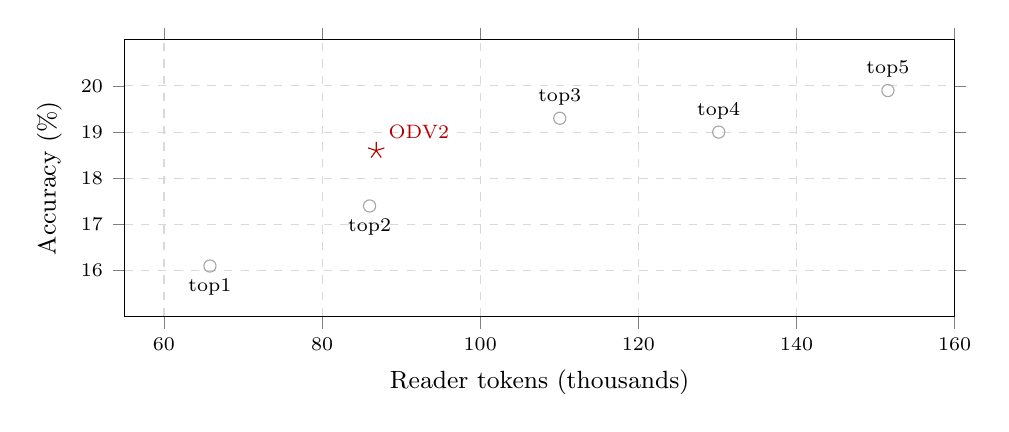
\begin{tikzpicture}
\begin{axis}[
    width=\columnwidth,
    height=5.1cm,
    xlabel={Reader tokens (thousands)},
    ylabel={Accuracy (\%)},
    xlabel style={font=\small},
    ylabel style={font=\small},
    xmin=55, xmax=160,
    ymin=15, ymax=21,
    xtick={60,80,100,120,140,160},
    ytick={16,17,18,19,20},
    xticklabel style={font=\scriptsize},
    yticklabel style={font=\scriptsize},
    grid=major, grid style={dashed, gray!30},
    tick align=outside,
    clip=false,
]
\addplot[only marks, mark=o, mark size=2.2pt, draw=gray!70, fill=gray!25]
coordinates {
    (65.812,16.1)
    (86.002,17.4)
    (110.058,19.3)
    (130.157,19.0)
    (151.558,19.9)
};
\addplot[only marks, mark=star, mark size=3.1pt, draw=red!70!black, fill=red!45]
coordinates {(86.838,18.6)};
\node[font=\scriptsize, anchor=north, yshift=-1.2pt] at (axis cs:65.812,16.1) {top1};
\node[font=\scriptsize, anchor=north, yshift=-1.2pt] at (axis cs:86.002,17.4) {top2};
\node[font=\scriptsize, anchor=south west, xshift=1.0pt, yshift=1.0pt, text=red!70!black] at (axis cs:86.838,18.6) {ODV2};
\node[font=\scriptsize, anchor=south, yshift=1.2pt] at (axis cs:110.058,19.3) {top3};
\node[font=\scriptsize, anchor=south, yshift=1.2pt] at (axis cs:130.157,19.0) {top4};
\node[font=\scriptsize, anchor=south, yshift=1.2pt] at (axis cs:151.558,19.9) {top5};
\end{axis}
\end{tikzpicture}
\caption{Accuracy--cost tradeoff. ODV2 compact is Pareto-efficient within the measured top-5 evidence budget: it operates near the top-2 reader-token budget while recovering part of the accuracy lost by naive top-2 truncation.}
\label{fig:token_reduction}
\end{figure}

\section{Discussion}

The current results support a narrower decomposition of agent memory into evidence recall and reader-budget control. Official Mem0 OSS supplies the retrieved evidence, while evidence-gated memory decides how much of that ranked evidence is passed to the frozen reader. The gate substantially reduces the amount of text read by the answerer, while accuracy is reported only as a guardrail. This distinction should remain central to the paper framing.

This framing matters for scalable agent systems. If every memory query requires passing many retrieved facts to a reader, long-horizon systems inherit a growing prompt-cost burden even when the backend can retrieve relevant evidence. The reported run shows that a lightweight post-retrieval gate can remove approximately three-fifths of retrieved context tokens under a fixed open-source Mem0 setup. The small accuracy drop should not be overinterpreted because absolute accuracy is near the floor in two categories. The current result is best used as a budgeted utility ablation: ODV2 compact reduces reader tokens per correct answer from 2{,}444 to 1{,}497, operates near the top-2 token budget, recovers four correct answers relative to top-2, and remains below top-3 in both token cost and accuracy.

The low absolute accuracy is also informative. It indicates that this run is not a reproduction of the published Mem0 platform benchmark configuration. In our setup, official Mem0 OSS retrieves five records and the compact gate returns two; the reader is a local Qwen-7B model scored by a strict local span-match proxy. Published Mem0 platform results use different infrastructure and much larger retrieval depths. The manual audit reinforces this interpretation: several wrong answers are better described as missing retrieved evidence than reader arithmetic failures. The proper comparison inside this paper is therefore paired and local: official Mem0 OSS versus the same Mem0 evidence after ODV2 compact gating.

\section{Limitations}

The main limitation is that the result does not show an accuracy improvement. Accuracy is not the target metric of the paper; it is a guardrail for the token-savings claim. We therefore do not claim that ODV2 beats Mem0, official Mem0, or the Mem0 platform on broad conversational QA. The defensible result is narrower: ODV2 compact is a lower-cost operating point that reduces reader tokens by 42.7\% and reader tokens per correct answer by 38.8\% relative to the top-5 official Mem0 baseline, while losing four aggregate correct answers.

Second, the baseline is the official open-source Mem0 package under a constrained retrieval budget, not the Mem0 managed platform and not the published top-50 or top-200 benchmark setting. The low absolute accuracy should be reported rather than hidden, but it should not be interpreted as a claim about Mem0 platform quality. The top-$k$ replay study covers $k \le 5$ from the completed run, but a stronger version should compare top-10, top-50, and top-200 retrieval to separate retrieval recall failures from reader failures.

Third, the compact gate currently uses a simple ranked top-two cap. This is useful for testing cost reduction, but it is not an optimized policy. The \texttt{official\_mem0\_top2} replay shows that much of the measured token reduction comes from truncation itself. A more complete ablation should compare query-adaptive gates, simple deduplication, stale-state suppression without compaction, and compaction without stale-state suppression. Fourth, token count is only one systems metric. It is a stable proxy for reader cost, but a deployment-grade SCALE systems result should add cache-free throughput, H100 memory, GPU utilization, energy, and wall-clock cost. Fifth, the revision classifier is deterministic and heuristic-based. Real deployments require learned or model-assisted consolidation for ambiguous updates, implicit corrections, and cross-modal evidence. Finally, the current experiments are text-only. The SCALE setting motivates multimodal agent memory, but this paper only tests the structured memory layer that a multimodal extraction system could feed.

\section{Conclusion}

ODV2 compact provides evidence that evidence-gated memory can substantially reduce the token budget of official Mem0 OSS retrieval. On 311 paired LongMemEval questions, it reduces reader total tokens by 42.7\% and retrieved context tokens by 59.1\%, while the accuracy guardrail changes from 19.9\% to 18.6\%. A naive \texttt{official\_mem0\_top2} replay reaches a similar token budget but lower accuracy, 17.4\%, while top-3 replay reaches 19.3\% at a larger budget. In cost-normalized terms, ODV2 reduces reader tokens per correct answer from 2{,}444 to 1{,}497. The main contribution is not a universal retriever or a new benchmark-leading memory system. It is a conservative evidence gate that substantially reduces the evidence passed to a frozen reader and identifies a lower-cost Pareto operating point within this constrained Mem0 OSS setup.

\section*{LLM/Agent Usage Disclosure}

LLM-based coding and writing tools were used to assist with implementation, result summarization, manuscript revision, and reviewer-style critique. The authors remained responsible for experiment execution, numerical results, claim selection, and final manuscript content.

\section*{Artifact Status}

The submitted repository includes the official Mem0 package runner, top-$k$ replay, token analysis, submission-check generation, cache-free reader benchmarking, oracle answer-context replay, and per-case JSONL diagnostics. The active run directory is \path{results/official_mem0_basecompact_full_20260502T072459Z}. The four category files contain 622 original rows, corresponding to 311 paired \texttt{official\_mem0}/\texttt{official\_mem0\_odv2\_selective} cases; the replay files add top-$k$ diagnostic rows for $k \in \{1,2,3,4\}$. Submission-check outputs are saved under \path{submission_checks/}, including bootstrap intervals, the reviewed 50-case manual audit and summary, state-guard isolation rows, oracle answer-context rows, and cache-free reader-system traces. Full auditability requires the completed per-case JSONL outputs, the cleaned LongMemEval input checksum, model revision identifiers, vLLM server configuration, and run diagnostics.

\section*{Reproducibility Commands}

The paper tables are regenerated from per-case JSONL outputs using the repository scripts named above. The completed run stores the exact command logs, diagnostics, top-$k$ replays, bootstrap summaries, manual-audit sample, cache-free reader benchmark, and oracle answer-context replay under the active result directory.

\FloatBarrier
\bibliographystyle{icml2026}
\bibliography{references}

\end{document}
